% ---------------------------------------------------------------------------
\subsection{Benchmark File Format}

We use plain \ascii\ text files for our format. The actual structure
of the file is not important for the interpretation. In principal, the
file could be written in a single line (with the exception of
comments, see below). For the potential human reader, a sensible
layout and a restriction to eighty columns are helpful. The definition
of terminal symbols and handling of comments and white spaces is
explained in Section~\ref{lexer}. Include files are explained in
Section~\ref{inclfiles}. 

In the following we format \ts{terminal symbols} in
\ts{typewriter} font and \nts{non-terminal symbols} in \nts{boldface}.
Grammar rules for non-terminal symbols are occasionally given in the
extended Backus Naur Form (EBNF), where \texttt{::=} has the meaning
of ``is defined as'', \texttt{|} separates two alternative choices,
\texttt{[]} encloses an optional part, and \verb|{}| encloses a
repetitive part (zero or more times).

The grammar and its reference parser implementation support the
feature to read a sequence of several benchmark files, for example,
concatenated together.  A benchmark file consists of four parts; a
magic token identifying the file format, a sequence of file header
options, a sequence of classifications, and a sequence of the objects
that define the benchmark content, e.g., polynomials, curves, or
surfaces. These sequences might be empty. Formally:
\medskip

\begin{ccTexOnly}
\begin{tabular}{lll@{\hspace{10mm}\ldots\ }l}
%  \nts{Input} & \ts{::=} & \multicolumn{2}{l}{\Open\ \nts{File} \Close}\\[\ebnfskip]
  \nts{Input} & \ts{::=} & \multicolumn{2}{l}{\nts{File}}\\[\ebnfskip]
  \nts{File}  & \ts{::=} & \nts{FileFormat} & see Section~\ref{headerformat}\\
              &          & \verb|{| \nts{FileHeaderOption} \verb|}| 
                                          & see Section~\ref{headeropt}\\
              &          & \verb|{| \nts{Classification} \verb|}|
                                          & see Section~\ref{classification}\\
              &          & \verb|{| \nts{Object} \verb|}|
                                          & see Section~\ref{grammar}
\end{tabular}
\end{ccTexOnly}
\begin{ccHtmlOnly}
<table>
<tr><td><b>Input</b></td><td>::=</td><td><b>File</b></td><td>&nbsp;</td></tr>
<tr><td><b>File</b></td><td>::=</td><td><b>FileFormat</b></td><td>... see Section <a href=""></a></td></tr>
<tr><td>&nbsp;</td><td>&nbsp;</td><td>{<b>FileHeaderOption</b>}</td><td>... see Section <a href=""></a></td></tr>
<tr><td>&nbsp;</td><td>&nbsp;</td><td>{<b>Classification</b>}</td><td>... see Section <a href=""></a></td></tr>
<tr><td>&nbsp;</td><td>&nbsp;</td><td>{<b>Object</b>}</td><td>... see Section <a href=""></a></td></tr>
</table>
\end{ccHtmlOnly}

We give a short example file that contains a single line segments. The
end points are given with homogeneous integer coordinates. A longer
example can be found in Section~\ref{longexample}.

\begin{verbatim}
# simple example with one random line segment
FileFormat( "AcsBenchmark", 0, 1 )
BenchmarkName( "Lines" ) 
Classification( "Arrangement", "Lines", "BoundedArcs", "Rnd", "2", "Sept-2004")
LineSegment_2( Point_2(1,1,1), Point_2(8,5,2))
\end{verbatim}

\subsection{Lexer Tokens, Comments, and White Spaces\label{lexer}}

A \verb|#| character starts a single-line comment up to the end of the
current line. 

\begin{alltt}
\ts{#} commentary text, or
Conic(1,2,3,4,5,6) \ts{#} commentary text until the end of the line
\end{alltt}

\noindent
Longer and also possibly nested comments stretching over multiple
lines can be enclosed with the keyword \ts{Comment(...)}, however,
parenthesis must match up properly:

\begin{alltt}
\ts{Comment(} commentary text (even nested)
         across multiple lines \ts{)}
\end{alltt}

\noindent
Comments and white spaces can be used everywhere in the file and are
ignored by the parser.

The lexical analyzer (lexer) detects all terminal symbols. Besides the
keywords, such as \ts{Comment}, these are numbers, strings, and the
constants \ts{VOID}, \ts{MINUS\_INFTY}, \ts{PLUS\_INFTY},
\ts{COUNTERCLOCKWISE}, and \ts{CLOCKWISE}. In particular we have:
\medskip

\begin{ccTexOnly}
\begin{tabular}{ll}
  \ts{INTEGER} &  integer number of arbitrary precision, may have a
  leading sign.\\[\ebnfskip]
  \ts{FNUMBER} &  floating point number in the usual scientific
  notation, but not an \ts{INTEGER}, \\ & and restricted to IEEE double
  precision. \\[\ebnfskip]
  \ts{STRING}  &  string in double quotes \ts{"..."}, may include
  newlines. The escape character \verb|\| \\ & can be used to represent
  double quotes within the string as \verb|\"|, or to represent\\ & the
  escape character itself in the string as \verb|\\|.
\end{tabular}
\end{ccTexOnly}

\subsubsection{IncludeFile\label{inclfiles}}

The file format and the reference parser implementation support
include files. They are not used in the current plans for benchmarks,
but they might turn out to be useful later for the hierarchical data
sets. A statement \ts{IncludeFile(}\textit{filename}\ts{)} instructs
the lexical scanner to stop scanning the current file and to continue scanning
the new file with the given \textit{filename}. Once the end of new
file has been reached, scanning resumes in the old file right after
the include statement. Include statements can be nested to an
arbitrary depth. An example:

\begin{verbatim}
IncludeFile( FullConicsRnd_10_1.arr)
\end{verbatim}

\subsubsection{FileFormat\label{headerformat}}

The mandatory \ts{FileFormat} field contains the \emph{magic-key\/}
string ``AcsBenchmark'' such that the parser recognizes that this file
is supposed to be a valid benchmark file.  The field also contains a
major and a minor version number. If the minor version number changes,
the parser with the same (or higher) major version number can still
process the file. If the major version number of the file is higher
than the major version number of the parser (fundamental modifications
in the format definition were made), the parser cannot read the format
any longer and throws an exception. An example:

\begin{verbatim}
FileFormat( "AcsBenchmark", 0, 1 )
\end{verbatim}

\subsubsection{FileHeaderOption\label{headeropt}}

Currently, only one file header option is specified, the
\ts{BenchmarkName}. It corresponds to the filename and reflects part
of the classification, see Section~\ref{classification}. One benefit
is that already the filename communicates the types of objects, how
many there are, which random number seed has been used, and if the
objects are randomized or degenerated. Grammar:

\begin{ccTexOnly}
\begin{tabular}{lll}
  \nts{FileHeaderOption} & \ts{::=} & \ts{BenchmarkName( STRING )}
\end{tabular}
\end{ccTexOnly}
\begin{ccHtmlOnly}
<table>
<tr><td><b>FileHeaderOption</b></td><td>::=</td><td><tt>BenchmarkName( STRING )</tt></td></tr>
</table>
\end{ccHtmlOnly}

\subsubsection {The Classification}
\label{classification}

The classification declares what types of objects appear in the
benchmark file. The classification is inspired by hierarchical
biological classifications. It consists of a sequence of string
arguments that go from the general to the specific properties of a
benchmark. Thus, the classification is subject to additions whenever a
new benchmark is devised. In particular, the number of properties
might not be the same for all classifications. However currently it
consists of six properties.  Note that such a tree-shaped
classification is not necessarily the only valid view on such a
classification problem, e.g., which property is more specific than
some other property. We also allow property entries to be undefined
and set to the empty string \ts{""}.
The classification with its dependencies is illustrated in
Figure~\ref{bench_fig::class}.

\begin{figure}[t]
\begin{ccTexOnly}
  \begin{center}
  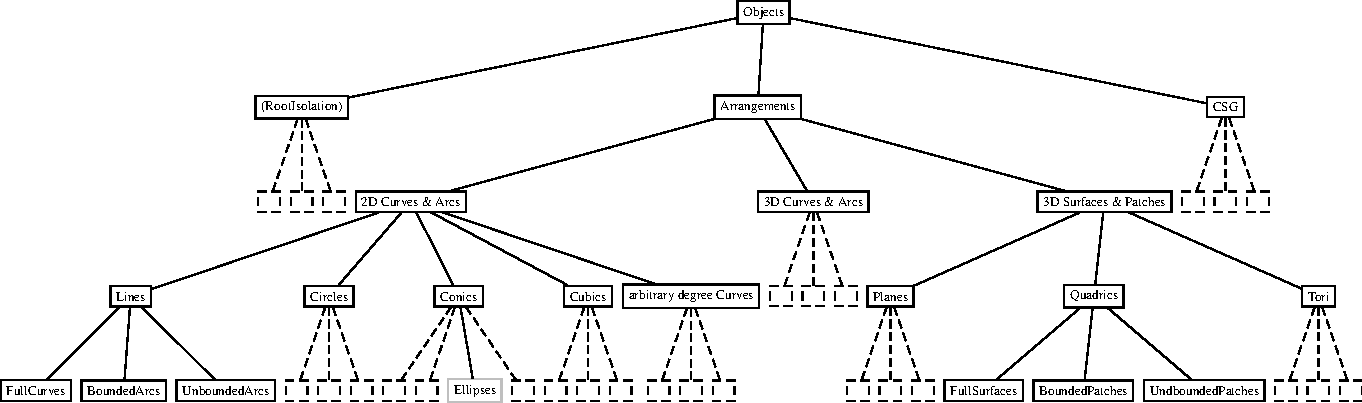
\includegraphics[width=\textwidth]{Benchmark/fig/classification}
  \end{center}
\end{ccTexOnly}
\begin{ccHtmlOnly}
  <p><center>
  <img src="./fig/classification.gif" border=0 alt="classification">
  </center>
\end{ccHtmlOnly}
\caption{Classification\label{bench_fig::class}}
\end{figure}

\begin{itemize}
  \item {\bf Problem:} the algorithmic problem that this benchmark
    addresses. Possible choices are \ts{"Arrangement"} for arrangement
    computations or \ts{"CSG"} for a constructive solid
    geometry Boolean operations evaluation problem. The filename
    suffix  depends on the problem. It is \ts{.arr} or \ts{.csg}
    correspondingly. Once ACS project members see further demands, 
    it can be easily extended.
  \item {\bf Geometry:} distinguishes between the 2D and 3D supporting
    geometric objects. In 2D the choices are \ts{"Lines"},
    \ts{"Circles"}, \ts{"Conics"}, \ts{"Cubics"}, \ts{"Quartics"}, and
    \ts{"arbitrary degree curves"}. In 3D the choices are 
    \ts{"Planes"}, \ts{"Quadrics"}, and \ts{"Tori"}.
  \item {\bf Class:} In 2D the choices are \ts{"FullCurves"},
    \ts{"BoundedArcs"}, and \ts{"UnboundedArcs"}, where unbounded arcs
    obviously also cover bounded arcs. For conics the class could
    additional be set to \ts{"Ellipses"}. In 3D the choices are
    \ts{"FullSurfaces"}, \ts{"BoundedPatches"}, and \ts{"UnboundedPatches"}. 
  \item {\bf Family:} specifies the specific property that
    characterizes this specific set of benchmark objects. For example,
    families of random objects are named \ts{"Rnd"} and families of
    degenerate objects are named \ts{"Dgn"}. 
  \item {\bf Instance:} extends the family to specific collection of
    benchmark object, for example, for a family of random objects by
    fixing the seed of the pseudo random number generator (thus
    specifying a deterministic sample of the random distribution).
  \item {\bf Revision:} contains the latest date when the benchmark was
    specified or modified. These modifications are expected to be
    infrequent, so we store just the month and year, such as in
    \ts{"May-2005"}. 
\end{itemize}

\noindent
The filename consists of the concatenation of the \nts{Geometry}, the
\nts{Class}, the \nts{Family}, the number of objects in the file, the
\nts{Instance}, and the suffix according to the \nts{Problem}.

Here is an example for a complete Classification:

% ??????
%Classification("Arrangement", "Conics", "FullCurves", "FullConicsRnd_30", 
%               "FullConicsRnd_30_2", "May-2005")

\begin{verbatim}
Classification("Arrangement", "Conics", "FullCurves", "Rnd", "2", "May-2005")
\end{verbatim}

\noindent
This classification example describes a benchmark file which contains
a sequence of random conics generated starting with a pseudo random
number generator seed 2. Assuming we have thirty conics in this file
then we get its corresponding filename as
\texttt{ConicsFullCurvesRnd\_30\_2.arr}. 
  
There can be more than one classification in a benchmark file, i.e., if
a single benchmark file contains a combination of different object types.
For example, a file containing circles, bounded conic arcs, and
ellipses, has the classification:

\begin{verbatim}
Classification("Arrangement", "Circles",  "FullCurves", "Rnd", "2", "May-2005")
Classification("Arrangement", "Conics",  "BoundedArcs", "Rnd", "2", "May-2005")
Classification("Arrangement", "Ellipses", "FullCurves", "Rnd", "2", "May-2005")
\end{verbatim}

\noindent
The classification must contain an entry for each distinct object
type, such that an application can rely on the classification to the
extend that if the classification mentions only conics but not
circles then the file does not contain \ts{"Circle\_2"} entries. Or
the other way around, if the application does not wish to handle
circles, it can issue an error message as soon as it sees the
classification mentioning circles. Note that of course mathematically
a conic can represent a circle as well, but this will not require the
classification to mention circles.

Finding a good filename for such a combined file might become difficult.
However, assuming we have sixty curves and arcs in this file, we could
suggest for a corresponding filename
\texttt{CirclesEllipsesFullCurvesConicsBoundedArcsRnd\_60\_2.arr}, and
it simplifies matters if the seed values are the same. In principle,
the filename could be shortened to express only commonalities of the
objects if it does not create conflicts with other filenames. For
example, combined data sets are likely to come from a specific example
or application and could have a common instance name, such as
\ts{"CgalLogo"} for the \cgal\ logo that consists of full circles and
line segments. Its filename could be shortened to
\texttt{CirclesCgalLogo\_92.arr}.

Combining different problems or different dimensions in one file does
not seem to make sense from our current perspective.
